\documentclass[a4paper, 12pt]{article}
\usepackage[english]{babel}
\usepackage[utf8]{inputenc}
\usepackage[T1]{fontenc}
\usepackage{lmodern}
\usepackage{hyperref}
\usepackage[numbers, sort&compress]{natbib}
\usepackage{calc}
\usepackage{fancyhdr}
\usepackage{graphics}
\usepackage{nowidow}
\usepackage{color}
\usepackage{subcaption}
\usepackage{enumitem}
\usepackage{epsfig}
\usepackage{epstopdf}
\usepackage{verbatim}


\newlength{\oneLine}
\newlength{\halfLine}
\setlength{\oneLine}{12pt}
\setlength{\halfLine}{6pt}

\newlength{\eqMargin}
\newlength{\eqHorizMargin}
\newlength{\eqVertMargin}

\setlength{\eqMargin}{20mm}
\setlength{\eqHorizMargin}{\eqMargin}
\setlength{\eqVertMargin}{\eqMargin}

% Paper
\setlength{\paperwidth}{210mm}
\setlength{\paperheight}{297mm}

% Rid the extra space
\setlength{\hoffset}{-1in}
\setlength{\voffset}{-1in}
\addtolength{\hoffset}{\eqHorizMargin}
\addtolength{\voffset}{\eqVertMargin}

% Set margin from the page border (horizontal)
\setlength{\oddsidemargin}{0pt}
\setlength{\evensidemargin}{0pt}

% Header
\setlength{\topmargin}{0pt}
\setlength{\headheight}{42pt}
\setlength{\headsep}{18pt}
\renewcommand{\headrulewidth}{0pt}

% Footer
\addtolength{\footskip}{18pt}
\renewcommand{\footrulewidth}{0pt}

% Margin notes
\setlength{\marginparsep}{0pt}
\setlength{\marginparwidth}{0pt}

% Text
\setlength{\textwidth}{\paperwidth - \hoffset - \hoffset - 25.4mm - 25.4mm}
\setlength{\textheight}{\paperheight - \voffset - \topmargin - \headheight - \headsep - \footskip - \voffset - 25.4mm - 25.4mm}

%\setlength{\labelwidth}{20mm}

% Hyperref settings
\hypersetup{
    unicode=true,					% non-Latin characters in Acrobat's bookmarks
    pdftoolbar=true,				% show Acrobat's toolbar?
    pdfmenubar=true,				% show Acrobat's menu?
    pdffitwindow=false,				% window fit to page when opened
    pdfstartview={FitH},			% fits the width of the page to the window
    pdftitle={S-26.3120 Radio Engineering, laboratory course},	% title
    pdfauthor={Tuomas Leinonen} {Sampo Salo} {Huy Nguyen},	% author
    pdfsubject={Radio Engineering},	% subject of the document
    pdfcreator={LaTeX},				% creator of the document
    pdfproducer={Aalto},			% producer of the document
    pdfkeywords={radio} {gsm} {bs} {tx},	% list of keywords
    pdfnewwindow=true,				% links in new window
    colorlinks=true,				% false: boxed links; true: colored links
    linkcolor=black,				% color of internal links
    citecolor=black,				% color of links to bibliography
    filecolor=black,				% color of file links
    urlcolor=black					% color of external links
}

% Bad hyphenation
%\hyphenation{}

% Macros
\newcommand{\dB}{\mathrm{\;dB}}
\newcommand{\dBm}{\mathrm{\;dBm}}
\newcommand{\m}[1]{\mathrm{#1}}

\definecolor{dkred}{rgb}{0.6, 0, 0}
\definecolor{dkgrn}{rgb}{0, 0.6, 0}
\definecolor{dkblue}{rgb}{0, 0, 0.6}

\pagestyle{fancy}
\lhead{S-26.3120 Radio Engineering, laboratory course\\Lab 2: GSM Base Station Receiver -- Pre-study report\\}
\rhead{Sampo Salo, 79543L\\Tuomas Leinonen, 84695P\\Huy Nguyen, 411330}
\cfoot{\thepage}


\begin{document}

\begin{titlepage}
\pagestyle{empty}
\begin{center}

\vspace*{30mm}
\noindent\LARGE{\textbf{S-26.3120 Radio Engineering, laboratory course}}

\vspace*{20mm}

\Large{\textbf{Lab 2: GSM Base Station Receiver}}\\

\vspace*{15mm}

\large{\textbf{Pre-study report}}\\
\vspace{15mm}
\large{\today}
	
\vspace*{30mm}
\large{
	\begin{tabular}{l l}
		\textbf{Group 3:} 	& \\
		Sampo Salo			& 79543L	\\
		Tuomas Leinonen 	& 84695P	\\
		Huy Nguyen			& 411330			
	\end{tabular}
}

\end{center}

\end{titlepage}

\section{Measurement and setup descriptions}

\textit{Present all the required measurement setups (draw a figure) 
and procedures. Take into account the attenuation of the cables. In 
which range is the attenuation of coaxial cables at 900~MHz? Pick 
the most suitable measurement equipment if there are several options 
to choose from.}

\vspace*{\oneLine}
\noindent
The figure on page 8 in \cite{hs} suggests that for a standard PE coax 
cables the attenuation ranges between $0.32 \ldots 1.36$~dB/m at a frequency 
of 900 MHz. Even lower losses may be achieved with more expensive cables 
(down to roughly 0.2~dB/m, as suggested on page 29 in \cite{hs}). Similarly, 
some maltreated cables may have an attenuation in excess of 2~dB/m. In 
addition, one should not overlook the attenuation from connectors and 
connecting.

When it comes to this lab course and our measurements, an attenuation 
of roughly 0.5~dB/m would most likely be a realistic estimate.


\subsection{1 dB compression point of the RX pre-amplifier block}

\textit{The compression point is a measure of maximum power at which 
the input amplifier works in linear mode and sets limit to the received 
signal power level. The frequency of 900 MHz is conveniently around the 
center of the RX band.}

\vspace*{\oneLine}
\noindent
The measurement setup suitable for this measurement is shown in Fig. \ref{f:m1}. 
A signal generator is used as a signal source, and the generated signal is passed 
through the DDU module before detection with a (precalibrated) spectrum analyzer. 
The input and output connections used in the DDU module are ANT and RX$_1$, 
respectively. An attenuator is used between the generator and the DDU module, 
if necessary. While the operator's manual of the R\&S SML03 signal generator 
does not explicitly mention the power range, the testing range defined in the 
\textit{Performance Tests} suggests a (reliable) minimum output power level 
of $-80$~dBm.

\begin{figure}[h!]
	\begin{center}
	\setlength{\unitlength}{1mm}
	\begin{picture}(167, 13)
		\linethickness{0.2mm}
		\put(0, 0.4){\framebox[34mm]{Signal generator}}
		\put(34, 1.4){\vector(1,0){14}}
		\put(48, 0){\framebox[23mm]{Attenuator}}
		\put(71, 1.4){\vector(1,0){14}}
		\put(85, 0.4){\framebox[28mm]{$\mathrm{ANT} \rightarrow \mathrm{RX}_1$}}
		\put(113, 1.4){\vector(1,0){14}}
		\put(127, 0.4){\framebox[40mm]{Sprectrum analyzer}}
		
		%\put(41, 4){\makebox(0,0){Cable}}
		%\put(78, 4){\makebox(0,0){Cable}}
		%\put(120, 4){\makebox(0,0){Cable}}
		\put(99, 7){\makebox(0,0){DDU module}}
		\put(66.5, 8){\makebox(0,0){$\overbrace{\hspace*{35mm}}^\textrm{if needed}$}}
	\end{picture}
	\vspace*{\halfLine}
	\caption{Measurement setup used in the first measurement task.}
	\label{f:m1}
	\end{center}
	\vspace*{-12pt}
\end{figure}

The measurement itself is basically a power sweep at a constant frequency of 
$f = 900$ MHz. We start off with a power level well above the receiver sensitivity 
level ($P_\mathrm{min,\;BS} \approx -112.5$~dBm), say $-100$~dBm. From there we 
gradually increase the power in suitable steps of $0.1 \ldots 10$~dB, depending on 
the current position on the $P_\mathrm{out}(P_\mathrm{in})$ transfer curve. That 
is, we'll start with a big step size and decrease it as we get close to the 
``sweet spot''. 

This power sweep is continued until we experience a compression of more than the 
required 1 dB. While one could just measure the input power required for the output 
to be 1 dB less than the expected value, this type of ``on-the-fly'' comparison 
is prone to error. Thus it's better to measure a full power sweep and leave the 
comparison to be done after the measurement and against a fitted straight representing 
ideal behaviour.

Since we are dealing with a GSM receiver, we may use the same settings for the 
spectrum analyzer as we did in the first labs -- except for the averaging factor. 
They were as follows: an averaging factor of 500, zero span and 30~Hz video and 
resolution bandwidths. An averaing factor of 500 would make the measurement quite 
lengthy, especially if dense power ``grid'' is used. Averaging over 100 measurements 
will most likely be more than adequate. Depending on the 1~dB compression point, 
we might need to watch out for compression in the spectrum analyzer. This is taken 
care of by altering the input attenuation.

The effect of the cables and the attenuator may be measured using a VNA (could be used 
for the entire measurement aswell), or using the SA by making the whole measurement 
relative. In a relative measurement, the power is measured again when the DDU module 
is by-passed to account only for the cables and the possible attenuator. This also 
required to know the real input power. 


\subsection{Gain of the RX pre-amplifier block}

\textit{The bandwidth of the RX block should account for the GSM specification 
for the RX band limits. Measure the 3~dB bandwidth of the block and determine 
approximately the equivalent noise bandwidth (graphically using the additional 
material) and the TX-band (stop band) attenuation.}

\vspace*{\oneLine}
\noindent
Wasn't this already covered in the first laboratory assignment as a part of the 
diplexer characterization? Fig. \ref{f:m2} presents the measurement setup used 
there. The DDU module is simply connected between the two ports of a precalibrated 
VNA; ANT and RX$_1$ connectors of the DDU module are connected to ports 1 and 2 of 
the VNA, respectively. In the VNA, measurement power shoud be as high as possible 
due the stop band-attenuation, yet simultaneously small enough not to cause 
compression in the pass-band (in neither the VNA nor in the pre-amp itself).

\begin{figure}[h!]
	\begin{center}
	\setlength{\unitlength}{1mm}
	\begin{picture}(126, 10)
		\linethickness{0.2mm}
		\put(0, 0.4){\framebox[29mm]{VNA (Port 1)}}
		\put(29, 1.4){\vector(1,0){20}}
		\put(49, 0.4){\framebox[28mm]{$\mathrm{ANT} \rightarrow \mathrm{RX}_1$}}
		\put(77, 1.4){\vector(1,0){20}}
		\put(97, 0.4){\framebox[29mm]{VNA (Port 2)}}
		
		%\put(39, 4){\makebox(0,0){Cable}}
		%\put(87, 4){\makebox(0,0){Cable}}
		\put(63, 7){\makebox(0,0){DDU module}}
	\end{picture}
	\vspace*{\halfLine}
	\caption{Measurement setup used when determining the gain of the pre-amplifier block.}
	\label{f:m2}
	\end{center}
	\vspace*{-12pt}
\end{figure}

The following figure (Fig. \ref{f:r1}) shows the results obtained in the first lab works 
with a transmit power of $-20$ dBm in the VNA (using the B-half of the BS and connecting 
the ports vice versa). In the figure, in addition to GSM RX and TX bands (in red), both 
3~dB (in blue) and noise (in green) bandwidth of the pre-amp block are visualized. This 
noise bandwidth visualization is somewhat questionable as it's a purely theoretical concept, 
but is nevertheless shown for scale. The shown noise bandwidth is found using a numerical 
approximation with $|S_{12}|$ of the formula given in the lecture supplement handout:

\begin{equation}
B_\mathrm{n} = \frac{1}{G_\mathrm{T,\;max}} \int_0^\infty G_\mathrm{T}(f) \, df.
\end{equation}

The noise bandwidth shown is less than the actual band since we cannot use infinite frequency 
range. Frequency range of $850 \ldots 1000$~MHz with $|S_{12}|_\mathrm{max} = 24.4$~dB 
was used instead. The obtained value (38.1~MHz) is roughly 6~\% shy of the 3~dB bandwidth 
(40.6~MHz), as one might expect. The 3~dB bandwidth may thus be used to avoid being 
overly optimistic.

\begin{figure}[h!]
	\begin{center}
	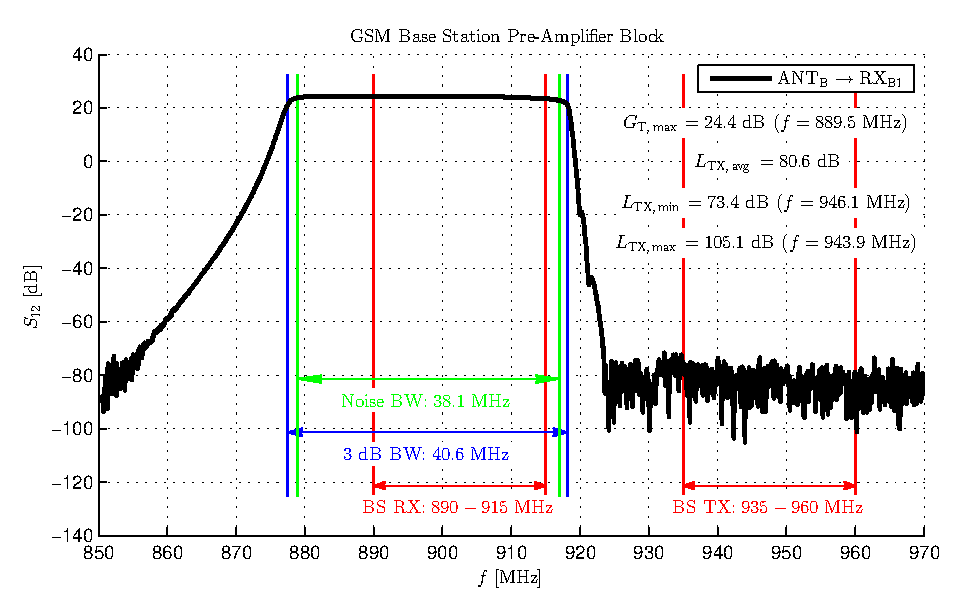
\epsfig{file=img/s12.eps, width=\textwidth}
	\caption{Results from the diplexer characterization.}
	\label{f:r1}
	\end{center}
	\vspace*{-12pt}
\end{figure}

In the graphical approximation method we need to investigate the effect of frequency 
roll-off speed. From Fig. \ref{f:r1} the transition bands are approx. 30~MHz (3.4 \%) 
and 5~MHz (0.55 \%) for lower and upper bands, respectively. During this transition, 
the $S_12$ drops roughly 100~dB from $+20$~dB to $-80$~dB. This corresponds to a slope 
of $3.3$~dB/MHz (29~dB/\%) and $-20$~dB/MHz ($-180$~dB/\%), respectively. The effect of 
such steep slopes are neglectable, and thus the 3~dB bandwidth may be used as the noise 
bandwidth.

If a VNA is not available as the instructions suggest, the task is quite laborious and 
absurd, just to be honest. Nevertheless, the procedure is listed here for completeness. 
We would need to simulate the VNA function manually using a signal generator and a power 
meter or a signal analyzer, leading to a setup like the one shown in Fig. \ref{f:m1}. The
output power is kept constant while frequency is swept over the range, taking notes on the 
relative power levels observed in the detector.


\subsection{Noise temperature of the RX pre-amplifier block}

\textit{Determine the noise temperature of the RX block (consisting of bias tee, 
diplexer and pre-amplifier) with the Y-coefficient method. Use the noise diode 
as active noise source (and as passive noise source at room temperature when 
supply voltage is switched off).}

\vspace*{\oneLine}
\noindent
In the third measurement task, we'll use a setup shown in Fig. \ref{f:m3}. 
A DC-voltage source is connected to a noise diode connected directly to the 
ANT-input in the pre-amplifier block. This direct connection is desirable as 
attenuation changes the noise temperature. The signal led from the RX$_1$ 
output to a spectrum analyzer. An LNA may be needed in between the DDU output 
and the spectrum analyzer, as the spectrum analyzer might not be sensitive 
enough for the cold noise source. See section \ref{s:noise} for details.

\begin{figure}[h!]
	\begin{center}
	\setlength{\unitlength}{1mm}
	\begin{picture}(166, 13)
		\linethickness{0.2mm}
		\put(0, 0.4){\framebox[10mm]{$V_\mathrm{DC}$}}
		\put(10, 1.4){\vector(1,0){9}}
		\put(19, 0){\framebox[25mm]{Noise diode}}
		\put(44, 1.4){\vector(1,0){24}}
		\put(68, 0.4){\framebox[28mm]{$\mathrm{ANT} \rightarrow \mathrm{RX}_1$}}
		\put(96, 1.4){\vector(1,0){9}}
		\put(105, 0.4){\framebox[12mm]{LNA}}
		\put(117, 1.4){\vector(1,0){9}}
		\put(126, 0.4){\framebox[40mm]{Sprectrum analyzer}}
		
		\put(5, 7){\makebox(0,0){On/Off}}
		%\put(20, 4){\makebox(0,0){Cable}}
		\put(56, 8){\makebox(0,0){Direct}}
		\put(56, 4){\makebox(0,0){connection}}
		%\put(118, 4){\makebox(0,0){Cable}}
		\put(81.5, 7){\makebox(0,0){DDU module}}
		\put(115.5, 8){\makebox(0,0){$\overbrace{\hspace*{19mm}}^\textrm{if needed}$}}
	\end{picture}
	\vspace*{\halfLine}
	\caption{Noise temperature measurement setup}
	\label{f:m3}
	\end{center}
	\vspace*{-12pt}
\end{figure}

%In room temperature, a matched load (an approximation in this case) outputs a noise power 
%of $-159$ dBm for a 30 Hz band. With a maximum gain of 24.4~dB and a total noise figure 
%of 3.9~dB, the expected noise level is around $-131$~dBm. This value is considerably 
%lower than the given sensitivity of the SA: $P_\mathrm{SA,\;min} < -125$~dBm when 
%$B_\mathrm{res.} = 30$~Hz. LNA could be used to boost the signal to a more appropriate 
%level as it's effect on the noise temperature could be compensated using the Friis' 
%noise formula.

The measurement itself is carried out measuring two power levels required in the 
Y-pa\-ram\-e\-ter; when the DC-voltage is off/shorted (``cold'') and on (``hot''). As 
for the SA settings, we are measuring noise at a single frequency (using zero-span): 
a very weak, random signal. Thus, input attenuator should be disabled, and minimum 
resolution bandwith used. A large averaging factor, say a thousand, is also beneficial. 
The measurement may take a few minutes, and it's OK; there's only two measurements 
to be made.


\subsection{Sensitivity of the RX pre-amplifier block}

\textit{Measure the sensitivity of the RX block using suitable equipment.}

\vspace*{\oneLine}
\noindent
In the sensitivity measurement, we're trying to measure the minimum input power at 
ANT input that results in a detectable signal above the noise floor in the ouput 
of the DDU module. For this, a measurement setup identical to the one used in the 
first task may be used, as is shown in the following figure (Fig \ref{f:m4}). This 
time though it's more than likely that an attenuator is required.

\begin{figure}[h!]
	\begin{center}
	\setlength{\unitlength}{1mm}
	\begin{picture}(167, 13)
		\linethickness{0.2mm}
		\put(0, 0.4){\framebox[34mm]{Signal generator}}
		\put(34, 1.4){\vector(1,0){14}}
		\put(48, 0){\framebox[23mm]{Attenuator}}
		\put(71, 1.4){\vector(1,0){14}}
		\put(85, 0.4){\framebox[28mm]{$\mathrm{ANT} \rightarrow \mathrm{RX}_1$}}
		\put(113, 1.4){\vector(1,0){14}}
		\put(127, 0.4){\framebox[40mm]{Sprectrum analyzer}}
		
		%\put(41, 4){\makebox(0,0){Cable}}
		%\put(78, 4){\makebox(0,0){Cable}}
		%\put(120, 4){\makebox(0,0){Cable}}
		\put(99, 7){\makebox(0,0){DDU module}}
		\put(66.5, 8){\makebox(0,0){$\overbrace{\hspace*{35mm}}^\textrm{if needed}$}}
	\end{picture}
	\vspace*{\halfLine}
	\caption{Measurement setup used in the sensitivity measurement.}
	\label{f:m4}
	\end{center}
	\vspace*{-12pt}
\end{figure}

The measurement starts be measing the noise floor at 900~MHz without any signal 
we're hoping to detect. That is, the RF power is switched off at the generator. 
Then we turn on an input signal that's some dBs sensitivity of $-112.5$~dBm. We 
gradually increase the power until the signal-to-noise ratio is no less than the 
10~dB required by the standard. One could also measure the power required to beat 
the noise just barely, and add the SNR later on if  $P_\mathrm{out}(P_\mathrm{in})$ 
relation is assumed to be ideal.

Since it's a GSM system, we use the measurement settings as they are defined in 
the standard. They are as follows: an averaging factor of 500, zero span and 30~Hz 
video and resolution bandwidths. As the spectrum analyzer input power is expected 
to be less than $-80$~dBm ($P_\mathrm{SA} \approx P_\mathrm{DDU,\;min} + G_\mathrm{DDU} = -112.5 \mathrm{\;dBm} + 24.4 \mathrm{\;dB}= -88.1 \mathrm{\;dBm}$), 
it's best to disable the input attenuator.


\newpage
\section{Pre-study calculations and related tasks}

The following subsections will present answers to pre-study tasks $2.2 - 2.4$.


\subsection{Mismatch attenuation}

\textit{A signal generator is connected to the input of the RX pre-amp block. 
The VSWR (voltage standing wave ratio) of the pre-amp is 2.0 and the VSWR of 
the output of the signal generator is 1.6.
\vspace*{-\halfLine}
\begin{enumerate}[label=\alph*), itemsep=0pt]
\item What is the range of additional attenuation due to this mismatch in 
	the measurement of the pre-amp block?
\item In what range is the attenuation due to mismatch, when an ideal 10 dB 
	attenuator is connected between the signal generator and the pre-amp block? 
	What is the benefit/drawback of inserting this attenuator?
\end{enumerate}}
		
\vspace*{\halfLine}
\noindent
Mismatch causes some of the source power to be reflected back from the load, 
reflecting again from the source. This way, the power from the source does not 
transfer fully to the load. The power attenuation $\eta$ due to mismatch is possible 
to be calculated using equations

\begin{equation}
\eta_\mathrm{SL,\;max} = \frac{(1 - |\rho_\mathrm{S}|^2)(1 + |\rho_\mathrm{L}|)^2}
	{1 - (|\rho_\mathrm{S}||\rho_\mathrm{L}|)^2}
\end{equation}

\noindent
and

\begin{equation}
\eta_\mathrm{SL,\;min} = \frac{(1 - |\rho_\mathrm{S}|^2)(1 + |\rho_\mathrm{L}|)^2}
{1 + (|\rho_\mathrm{S}||\rho_\mathrm{L}|)^2},
\end{equation}

\noindent
where $\rho_\mathrm{S}$ and $\rho_\mathrm{S}$ are the source and load reflection 
coefficients, respectively. The equations are special forms of an equation, and are 
used in the case when the phase relation of the set-up is not known. The reflection 
coefficients can be calculated from voltage standing wave ratio 
$\mathit{VSWR}$ by 

\begin{equation}
|\rho| = \frac{1 - \mathit{VSWR}}{1 + \mathit{VSWR}}.
\end{equation} 
\noindent
Using the equations, the maximum efficiency of power is $\eta_\mathrm{SL,\;max} 
= -0.14$ dB, and the minimum efficiency of power transfer is 
$\eta_\mathrm{SL,\;min} = -1.10$~dB. Therefore, the range of mismatch attenuation 
is $-1.10 \ldots {-0.14}$~dB.

With the attenuator in between, the reflections are attenuated 20 dB each time 
the power travels back and forth in between the source and the load. The 
attenuation for the reflections grows relatively large, and so the maximum 
efficiency of power can be approximated using an equation that is derived for 
a set-up where an isolator is placed between the source and the load. The equation 
is

\begin{equation}
\eta = (1 - |\rho_\mathrm{S}|^2)(1 + |\rho_\mathrm{L}|)^2,
\end{equation}

\noindent
and it gives an power attenuation of $-0.63$~dB. The advantage of using a power 
attenuator in between the source and the load is that the attenuation due to 
mismatch can be approximated more precisely. On the other hand, the total 
attenuation grows to $-10.6$~dB, which could be a big drawback for some 
measurements.


\subsection{Noise temperature}
\label{s:noise}

\textit{The noise temperature of the pre-amp block is determined using the 
Y-coefficient method. The noise level of the spectrum analyzer HP8596E is 
$P_\mathrm{SA} < -125$~dBm when the input is matched and the resolution 
bandwidth is 30~Hz.
\vspace*{-\halfLine}
\begin{enumerate}[label=\alph*), itemsep=0pt]
\item How much gain is required from the LNA in order to measure the noise 
	temperature with the HP8596E? The noise figure of the amplifier is 2.8~dB 
	and the attenuation of the bias tee and the diplexer is 0.7~dB and 0.4~dB, 
	respectively.
\item Does the order (i.e. which is first in the chain) of the amplifier, 
	bias tee and the diplexer in the pre-amp block have any influence on the 
	result of Y-coefficient measurement? If yes, say why.
\end{enumerate}}

\vspace*{\halfLine}
\noindent
The receive path of the DDU module, also referred to as the pre-amp block, 
consists of a bias tee, diplexer, LNA and a four-way power-divider (in this 
order). Assuming physical operating temperature of the pre-amp block to be 
$T_0 = 290$~K, we have the attenuations and noise factors/figures listed in 
the following table (Table \ref{t:c2}).

\begin{table}[!h]
	\begin{center}
	\caption{Given parameters for this problem.}
	\label{t:c2}
	\renewcommand*{\arraystretch}{1.2}
	\begin{tabular}{lccc}
	\textbf{Block} 			& \textbf{Subscript}	& \textbf{Attenuation} $L$ 	& \textbf{Noise figure} $F$ \\
	\hline
	Bias tee				& BT					& $0.7 \dB \approx 1.175$	& $0.7 \dB \approx 1.175$ \\
	Diplexer				& DPX					& $0.4 \dB \approx 1.096$	& $0.4 \dB \approx 1.096$ \\
	Low-noise amplifier		& LNA					& ???						& $2.8 \dB \approx 1.905$ \\
	4-way power divider		& DIV					& $6.0 \dB \approx 3.981$	& $6.0 \dB \approx 3.981$
	\end{tabular}
	\end{center}
	\vspace*{-12pt}
\end{table}

The total noise figure of a cascaded system $F_\mathrm{T}$ is given by the 
Friis noise equation (linear quatities)

\begin{equation} \label{e:f}
F_\mathrm{T} = F_1 + \frac{F_2 - 1}{G_1} + \frac{F_3 - 1}{G_1 G_2} + \frac{F_4 - 1}{G_1 G_2 G_3} + \cdots,
\end{equation}

\noindent
or equivalently using noise powers

\begin{equation}
F_\mathrm{T} = \frac{\mathit{SNR}_\mathrm{in}}{\mathit{SNR}_\mathrm{out}} 
	= \frac{S_\mathrm{in}}{N_\mathrm{in}} \, \frac{N_\mathrm{out}}{S_\mathrm{out}}
	= \frac{N_\mathrm{out}}{G_\mathrm{T} N_\mathrm{in}}
	= \frac{N_\mathrm{out}}{G_\mathrm{T} \, k T_0 B_\mathrm{N}}.
\end{equation}

\noindent
Solving for $N_\mathrm{out}$ yields

\begin{equation}
N_\mathrm{out} = F_\mathrm{T} \, G_\mathrm{T} \, k T_0 B_\mathrm{N} 
	= F_\mathrm{T} \, \frac{G_\mathrm{LNA}}{L_\mathrm{BT} L_\mathrm{DPX} L_\mathrm{DIV}} \, k T_0 B_\mathrm{N}
\end{equation}

\noindent
which can in turn to be solved for required gain $G_\mathrm{LNA}$ when we set 
$N_\mathrm{out} > P_\mathrm{SA,\;min}$. Thus we obtain

\begin{equation} \label{e:g}
G_\mathrm{LNA} > \frac{P_\mathrm{SA,\;min} \, L_\mathrm{BT} \, L_\mathrm{DPX} \, L_\mathrm{DIV}}%
	{F_\mathrm{T} \, k T_0 B_\mathrm{N}}.
\end{equation}

\vspace*{\oneLine}
\noindent
\textbf{a)} First we need to find the total noise figure of our four-stage cascaded system. 
Using Eq. \ref{e:f}, it is found to be
\begin{equation} \label{e:f2}
F_\mathrm{T} = 2.533 + \frac{3.840}{G_\m{LNA}}.
\end{equation}

\noindent
Using this in Eq. \ref{e:g} yields
\begin{equation} \label{e:g2}
G_\mathrm{LNA} > 5624.69 \ldots = 37.500 \ldots \dB \approx 37.5 \dB.
\end{equation}

This assumes the output of the DDU module ($RX_1$) to be perfectly matched 
to the spectrum analyzer. If we were to neglect the power divider 
($L_\m{DIV} = F_\m{DIV} = 1 = 0 \dB$), a gain of 31.5~dB would 
be required from the LNA.

\vspace*{\oneLine}
\noindent
\textbf{b)} From Eq. \ref{e:f} it can be observed that the noise figure of a 
system is dominated by the noise figure of the first stage since the effect of 
the following stages are reduced by the several gains. That is, if the first 
stage has a significant gain, the overall system noise figure more or less 
depends on the noise characteristics of the stage in question. Thus, if the 
order in the pre-amp block changes, it will definitely have influence on the 
noise temperature of the block.


\subsection{Requirements with evolving standards}

\textit{Discuss briefly the major changes in the requirements for the 
RF performance of the blocks in the RX chain when we move from 2G to 
3G to 4G systems.}

\vspace*{\oneLine}
\noindent
Write (at least) these out in a table and conclusions -like manner, for example.

More frequency bands, higher bandwidth, modulation methods, sensitivity, 
linearity requirements, carrier aggregation, multiaccess method, FDD/TDD

\begin{table}[!h]
	\begin{center}
	\caption{[WORK IN PROGRESS] A simplified list of some of the key requirements in evolving communication systems.}
	\label{t:234g}
	\renewcommand*{\arraystretch}{1.2}
	\begin{tabular}{lccc}
	\textbf{Parameter}				& \textbf{2G (GSM)}		& \textbf{3G (UMTS)} 	& \textbf{4G (LTE-A)} \\
	\hline
	System frequency [MHz]			& $820 \ldots 1990$		& $B \ldots B$			& $C \ldots C$	 \\
	Number of system bands			& 4						& B						& C	 \\
	System bandwidth [MHz]			& $25 \ldots 95$		& $B \ldots B$			& $C \ldots C$	 \\
	Channel bandwidth [MHz]			& 0.200					& $B \ldots B$			& $C \ldots C$	 \\
	Multiple-access method			& TDMA					& WCDMA					& OFDMA	 \\
	Duplexing mode					& TDD					& FDD					& FDD/TDD	 \\
	Modulation schemes				& GSMK					& QPSK					& QAM	 \\
	Sensitivity	req.				& A						& B						& C	 \\
	Linearity req.					& A						& B						& C	
	\end{tabular}
	\end{center}
	\vspace*{-12pt}
\end{table}


\begin{thebibliography}{9}%\itemsep 7pt\parskip -5pt 

\bibitem{hs} $\mathrm{Huber}+\mathrm{Suhner}$, 
	\textit{RF Cables}, 
	Edition 2013/09. 
	Available online at \href{http://ipaper.ipapercms.dk/HUBERSUHNER/Technologies/Radiofrequency/RFCablesEN/}
		{\texttt{http://ipaper.\linebreak{}ipapercms.dk/HUBERSUHNER/Technologies/Radiofrequency/RFCablesEN/}}
	[Retrieved: January 10th, 2014].

%\bibitem{pozar} D.\ M.\ Pozar, 
%	\textit{Microwave Engineering}, 
%	J.\ Wiley \& Sons, 4th Ed., 2012. 
%	ISBN: 978-0-470-63155-3.
	
%\bibitem{gains} J.\ C.\ Logan, J.\ W.\ Rockway, 
%	``Dipole and Monopole Antenna Gain and Effective Area for Communication Formulas.''
%	Available online at \url{www.dtic.mil/cgi-bin/GetTRDoc?AD=ADA332891}
%	[Retrieved: November 25th, 2013].

%\bibitem{parts} M.\ Steer, 
%	\textit{Microwave and RF Design -- A Systems Approach}, 
%	SciTech Publishing, 2010. 
%	ISBN: 978-1-891-12188-3.
	
%\bibitem{kandi} T.\ Leinonen, 
% 	``Antenna and front-end challenges for mobile software-defined radio receiver,''
%	B.\ Sc.\ (Tech.) thesis (in Finnish), 2012. 
% 	Available online at \url{http://urn.fi/URN:NBN:fi:aalto-201301161154}.
	
%\bibitem{iet} R.\ J.\ Collier, A.\ D.\ Skinner (editors), 
%	\textit{Microwave Measurements}, 
%	The Institution of Engineering and Technology, 3rd Ed., 2007. 
% 	ISBN: 978-0-86341-735-1.

\end{thebibliography}

\end{document}
